\subsection{Chapter 7 - Work and energy}

\subsubsection{Overview}\label{chap:workenergy}

In this chapter, we introduce a new way to build models derived from Newton's theory of classical physics. We will introduce the concepts of work and energy, which will allow us to model situations using scalar quantities, such as energy, instead of vector quantities, such as forces. It is important to remember that even when we are using energy and work, these tools are derived from Newton's Laws; that is, we may not be using Newton's Second Law explicitly, but the models that we develop are still based on the same theory of classical physics.

\begin{framed}
\textbf{Learning Objectives}\\
\begin{itemize}
\item Understand the concept of work and how to calculate the work done by a force.
\item Understand the concept of the net work done on an object and how that relates to a change in speed of the object.
\item Understand the concept of kinetic energy and where it comes from.
\item Understand the concept of power.
\end{itemize}
\end{framed}

\begin{framed}
\textbf{Think About It}\\
You are holding a heavy book with your arm extended horizontally. The book does not move as you struggle to keep it from falling to the ground. Does your arm do work on the book? If you start walking to class while holding the book, does your arm do work on the book?

\begin{framed}
\textbf{Answer}\\
Your arms do no work on the book. There is no displacement (the book does not move up or down), so you do no work, even if its tiring! If you are walking, the displacement is perpendicular to the force applied by your arms, your arms do no work.
\end{framed}
\end{framed}

\subsubsection{Work}

\begin{framed}
\textbf{Review}\\
\begin{itemize}
\item Section~\ref{sec:Vectors:scalarproduct} on the scalar product.
\item Section~\ref{sec:calculus:integrals} on integrals.
\end{itemize}
\end{framed}

We introduce the concept of work as the starting point for building models using energy instead of forces. Work is a scalar quantity that is meant to represent how a force exerted on an object over a given distance results in a change in speed of that object. We will first introduce the concept of work done by a force on an object, and then look at how work can change the kinematics of the object. This is analogous to how we first defined the concept of force, and then looked at how force affects motion (by using Newton's Second Law, which connected the concept of force to the acceleration of the object).

The work done by a force, $\vec F$, on an object over a displacement, $\vec d$, is defined to be:
\begin{equation}
\boxed{W = \vec F \cdot \vec d = Fd\cos\theta = F_xd_x+F_yd_y+F_zd_z}
\end{equation}
where $\theta$ is the angle between the vectors when they are placed tail to tail, as in Figure~\ref{fig:workenergy:fddotproduct}. The dimension of work, force times displacement, is also called ``energy''. The S.I. unit for energy is the Joule (abbreviated $\text{J}$) which is equivalent to $\text{Nm}$ or ${\rm kg m^2/s^2}$ in base units.

\begin{figure}[!htbp]
\centering
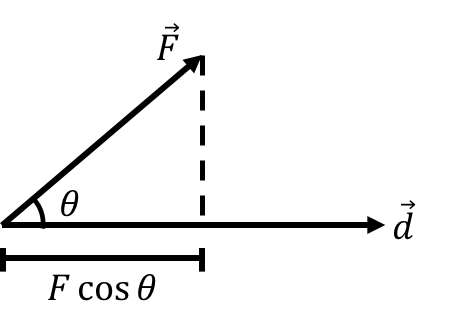
\includegraphics[width=0.3\linewidth]{files/fddotproduct-49904090da9ae6fe24ebcc94657f47b1.png}
\caption[]{When determining the scalar product $\vec F\cdot \vec d = Fd\cos\theta$, $\theta$ is the angle between the vectors when they are placed tail to tail.}
\label{fig:workenergy:fddotproduct}
\end{figure}

The work ``done'' by the force is the scalar product of the force vector and the displacement vector of the object. We say that the force ``does work'' if it is exerted while the object moves (has a displacement vector) and in such a way that the scalar product of the force and displacement vectors is non-zero. A force that is perpendicular to the displacement vector of an object does no work (since the scalar product of two perpendicular vectors is zero).  A force exerted in the same direction as the displacement will do positive work ($\cos\theta$ positive), and a force in the opposite direction of the displacement will do negative work ($\cos\theta$ negative). As we will see, positive work corresponds to increasing the speed of the object, whereas negative work corresponds to decreasing its speed. No work corresponds to no change in speed (but could corresponds to a change in velocity).

\begin{framed}
\textbf{Checkpoint}\\
A pendulum of length $R$ consists of a mass connected to a string (Figure~\ref{fig:workenergy:pendulumtension}). The string exerts a force of tension $\vec F_T$ on the mass. What is the work done by tension when the pendulum swings through an angle $\theta$?

\begin{figure}[!htbp]
\centering
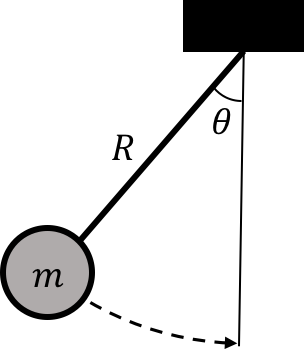
\includegraphics[width=0.2\linewidth]{files/pendulumworktension-a90b632f802628285c5f3f9cc394dcae.png}
\caption[]{A pendulum swings through an angle $\theta$.}
\label{fig:workenergy:pendulumtension}
\end{figure}

\begin{enumerate}
\item $W=F_TR\theta$
\item $W=F_TR(1 -\cos\theta)$
\item Tension does no work on the mass.
\end{enumerate}

\begin{framed}
\textbf{Answer}\\
\begin{enumerate}[resume]
\item
\end{enumerate}
\end{framed}
\end{framed}

You may be tempted to ask, ``Why work? Why not something else? Why that scalar product in particular? How could we possibly have thought of that?''. In general, it seems arbitrary that we introduce the quantity ``work'' and then find that it leads to a convenient way of building models. However, we did not just pull this quantity out of thin air! Many theorists, over many years, tried all sorts of quantities and ways to rephrase Newton's Theory that were not helpful. The quantities that make it into textbooks are the ones that turned out to be useful. You should also keep in mind that, just like force, work is a ``made-up'' mathematical tool that is helpful in describing the world around us. There is no such thing as work or energy; they are just useful mathematical tools.

\paragraph{Work in one dimension.}

Work involves vectors, so we can first examine the concept in one dimension, before extending this to two and three dimensions. We can choose $x$ as the coordinate in one dimension, so that all vectors only have an $x$ component. We can write a force vector as $\vec F=F\hat x$, where $F$ is the $x$ component of the force (which could be positive or negative). A displacement vector can be written as $\vec d = d \hat x$, where again, $d$ is the $x$ component of the displacement, and can be positive or negative. In one dimension, work is thus:
\begin{equation}
W = \vec F \cdot \vec d = (F\hat x) \cdot ( d\hat x ) = Fd (\hat x\cdot\hat x)=Fd
\end{equation}
where $\hat x \cdot \hat x = 1$. Consider, for example, the work done by a force, $\vec F$, on a box, as the box moves along the $x$ axis from position $x=x_0$ to position $x=x_1$, as shown in Figure~\ref{fig:workenergy:work1d}.

\begin{figure}[!htbp]
\centering
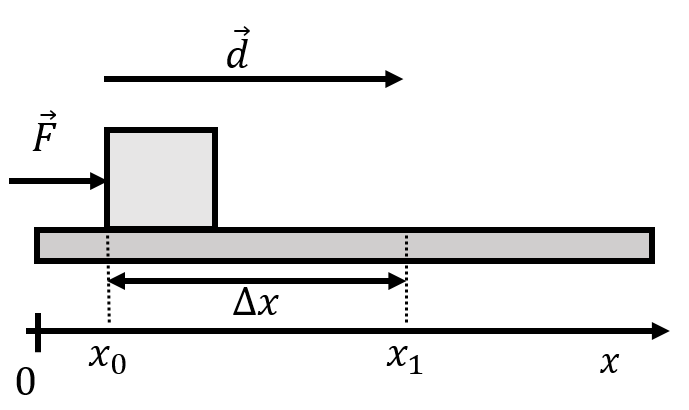
\includegraphics[width=0.4\linewidth]{files/work1d-0daf97b5d5589ef1f3195ed30fc5eb42.png}
\caption[]{A force, $\vec F$, exerted on an object as it moves from position $x=x_0$ to position $x=x_1$.}
\label{fig:workenergy:work1d}
\end{figure}

We can write the length of the displacement vector as $||\vec d|| =d= \Delta x = x_1 -x_0$. The work done by the force is given by:
\begin{equation}
W = \vec F \cdot \vec d = F\hat x\cdot \Delta x\hat x =F\Delta x =F(x_1-x_0)
\end{equation}
which is a positive quantity, since $x_1 > x_0$, with our choice of coordinate system.

\begin{framed}
\textbf{Checkpoint}\\
A constant force in the positive $x$ direction, $\vec F$, acts on a box, as in Figure~\ref{fig:workenergy:work1d}. Consider the work done by $\vec F$ as the box moves from $x_1$ to $x_0$. How does it compare to the work done by $\vec F$ when moving from $x_0$ to $x_1$ (that we calculated above)?

\begin{enumerate}
\item $\vec F$ does no work on the box when it moves from $x_0$ to $x_1$.
\item The work has the same magnitude as before, but the work is now negative.
\item The work done by $\vec F$ is the same in both cases.
\end{enumerate}

\begin{framed}
\textbf{Answer}\\
\begin{enumerate}[resume]
\item
\end{enumerate}
\end{framed}
\end{framed}

\paragraph{Work in one dimension - varying force}

Suppose that instead of a constant force, $\vec F$, we have a force that changes with position, $\vec F(x)$, and can take on three different values between $x=x_0$ and $x=x_3$:
\begin{equation}
  \vec F (x)=
  \begin{cases}
    F_1\hat x & x<\Delta x \\
    F_2\hat x & \Delta x \leq x< 2\Delta x \\
    F_3\hat x & 2\Delta x \leq x
  \end{cases}
\end{equation}
as illustrated in Figure~\ref{fig:workenergy:work1d}, which shows the force on an object as it moves from position $x=x_0$ to position $x=x_3$, along three (equal) displacement vectors, $\vec d_1=\vec d_2=\vec d_3=\Delta x \hat x$.

\begin{figure}[!htbp]
\centering
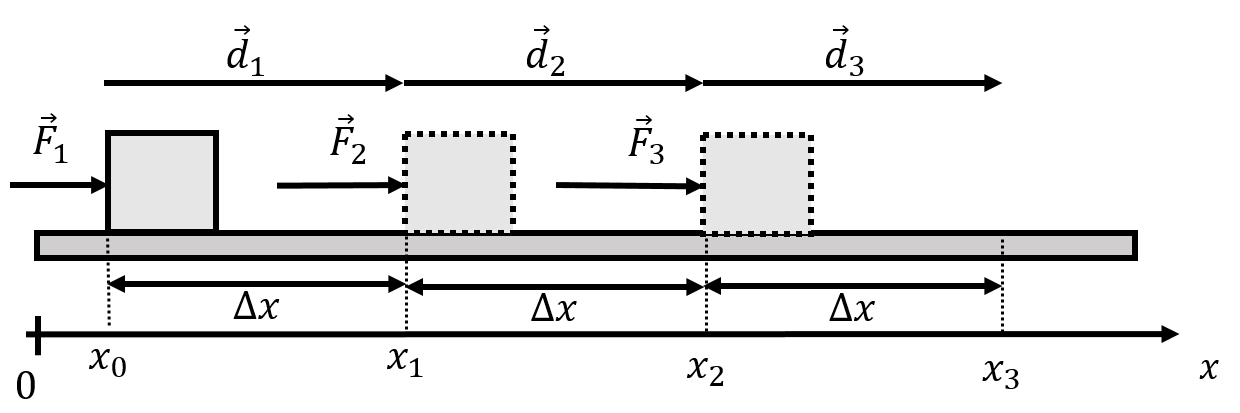
\includegraphics[width=0.7\linewidth]{files/work1dvarying-1dbde50e5bef34689b7c939f0392c213.png}
\caption[]{A varying force, $\vec F(x)$, exerted on an object as it moves from position $x=x_0$ to position $x=x_3$.}
\label{fig:workenergy:work1dvarying}
\end{figure}

The total work done by the force over the three separate displacements is the sum of the work done over each displacement:
\begin{equation}
W^{tot}&=W_1+W_2+W_3\\
&=\vec F_1\cdot \vec d_1+\vec F_2\cdot \vec d_2+\vec F_3\cdot \vec d_3\\
&= F_1\Delta x +F_2\Delta x + F_3\Delta x
\end{equation}

If instead of 3 segments we had $N$ segments and the $x$ component of the force had the $N$ corresponding values $F_i$ in the $N$ segments, the total work done by the force would be:
\begin{equation}
W^{tot} = \sum_{i=0}^N\vec F_i \cdot \Delta \vec x
\end{equation}
where we introduced a vector $\Delta \vec x$ to be the vector of length $\Delta x$ pointing in the positive $x$ direction. In the limit where $\vec F(x)$ changes continuously as a function of position, we take the limit of an infinite number of infinitely small segments of length $dx$, and the sum becomes an integral:
\begin{equation}
\boxed{W^{tot} = \int_{x_0}^{x_f}\vec F(x) \cdot d\vec x}
\end{equation}
where the work was calculated in going from $x=x_0$ to $x=x_f$, and $d\vec x=dx\hat x$ is an infinitely small displacement vector (of length $dx$) in the positive $x$ direction.

\begin{framed}
\textbf{Example 7.1}\\
A block is pressed against the free end of a horizontal spring with spring constant, $k$, so as to compress the spring by a distance $D$ relative to its rest length, as shown in Figure~\ref{fig:workenergy:spring}. The other end of the spring is fixed to a wall. What is the work done by the spring force on the block in going from $x= -D$ to $x=0$? What is the work done by the block on the spring over the same displacement?

\begin{figure}[!htbp]
\centering
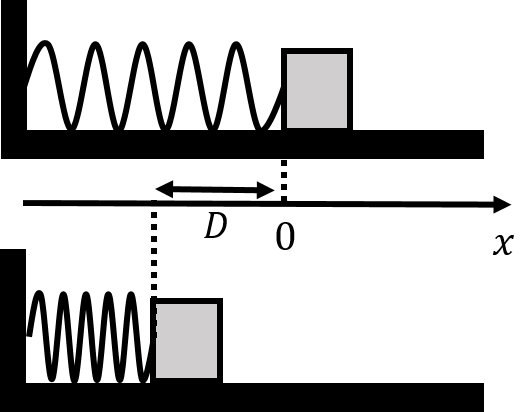
\includegraphics[width=0.4\linewidth]{files/spring-fb0b7b45895ba1ffc941557cc6a32aee.png}
\caption[]{A block is pressed against a horizontal spring so as to compress the spring by a distance $D$ relative to its rest length.}
\label{fig:workenergy:spring}
\end{figure}

\begin{framed}
\textbf{Solution}\\
The force exerted by the spring on the block changes continuously with position, according to Hooke's law:
\begin{equation}
\vec F(x) = -kx \hat x
\end{equation}
and points in the positive $x$ direction when the end of the spring has a negative $x$ position (with our coordinate choice illustrated in Figure~\ref{fig:workenergy:spring}, where the origin is located at the rest length of the spring). To calculate the work done by the force, we sum the work done by the force over many infinitesimally small displacements $d\vec x$ (using an integral):
\begin{equation}
W &= \int_{-D}^0 \vec F(x) \cdot d\vec x\\
&=\int_{-D}^0 (-kx \hat x) \cdot (dx \hat x)\\
&=\int_{-D}^0 -kxdx (\hat x \cdot \hat x)\\
&=-\int_{-D}^0 kx dx\\
&=-\left[\frac{1}{2}kx^2  \right]_{-D}^0\\
&=\frac{1}{2}kD^2
\end{equation}
In order to determine the work that was done by the block on the spring, we need to determine the force, $\vec F'(x)$, exerted by the block on the spring. By Newton's Third Law, this is equal in magnitude but opposite in direction to the force exerted by the spring on the block:
\begin{equation}
\vec F'(x) = -\vec F(x) = kx \hat x
\end{equation}
The work done by the block on the spring over the same displacement is:
\begin{equation}
W' &= \int_{-D}^0 \vec F'(x) \cdot d\vec x\\
&=\int_{-D}^0 (kx \hat x) \cdot (dx \hat x)\\
&=\int_{-D}^0 kx dx=-\frac{1}{2}kD^2\\
\end{equation}
which is negative. This makes sense because the force exerted by the block on the spring is in the direction opposite to the direction of displacement, so the work should be negative.
\end{framed}
\end{framed}

\paragraph{Work in multiple dimensions}

First, consider the work done by a force $\vec F$ in pulling a crate over a displacement $\vec d$, in the case where the force is directed at an angle $\theta$ above the horizontal, as shown in Figure~\ref{fig:workenergy:workangle}, and the displacement is along the $x$ axis (or rather, we chose the $x$ axis to be parallel to the displacement).

\begin{figure}[!htbp]
\centering
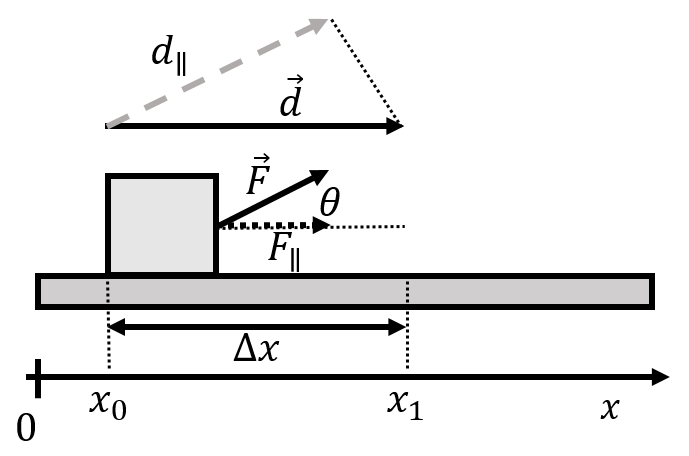
\includegraphics[width=0.5\linewidth]{files/workangle-c0fee3c95b822c28de3d889be8fac4c3.png}
\caption[]{A force, $\vec F$, exerted on an object as it moves from position $x=x_0$ to position $x=x_1$.}
\label{fig:workenergy:workangle}
\end{figure}

The work done by the force is given by:
\begin{equation}
W = \vec F \cdot \vec d &= Fd\cos\theta\\
&= F_{\parallel}d\\
&= Fd_{\parallel}\\
\end{equation}
where we highlighted the fact that the scalar product ``picks out'' components of vectors that are parallel to each other. $F_{\parallel} = F\cos\theta$ is the component of $\vec F$ that is parallel to $\vec d$, and $d_{\parallel}=d\cos\theta$ is the component of $\vec d$ that is parallel to $\vec F$. These are also shown in Figure~\ref{fig:workenergy:workangle}.

\begin{framed}
\textbf{Checkpoint}\\
Brent and Dean pull two crates by using ropes that make the same angle above the horizontal and with the same force. The magnitude of the crates' displacement is the same, but Dean's crate moves horizontally on the ground while Brent's crate moves up a frictionless ramp that is parallel to the rope used to pull the crate. Who did more work on the crate?

\begin{enumerate}
\item Dean because there is friction between his crate and the ground.
\item Brent.
\item They did the same amount of work.
\end{enumerate}

\begin{framed}
\textbf{Answer}\\
\begin{enumerate}[resume]
\item
\end{enumerate}
\end{framed}
\end{framed}

In general, if an object is moving along an arbitrary path, we cannot choose the $x$ axis to be parallel to the displacement or to the force. If the path can be sub-divided into straight segments over which the force is constant, as in Figure~\ref{fig:workenergy:work2d}, we can calculate the work done by the force over each segment and add the work done in each segment together to obtain the total work done by the force. Note that, in general, the work done by a force as an object moves from one position to another depends on the particular path that was taken between the two positions, since different paths will have difference lengths.

\begin{figure}[!htbp]
\centering
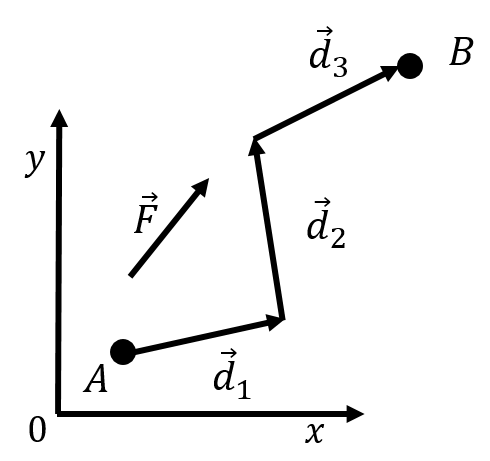
\includegraphics[width=0.4\linewidth]{files/work2d-99959f9f04f1f717440b6952780f6dab.png}
\caption[]{An arbitrary two dimensional path of an object from $A$ to $B$ broken into three straight segments.}
\label{fig:workenergy:work2d}
\end{figure}

\begin{framed}
\textbf{Example 7.2}\\
Compare the work done by the force of kinetic friction in sliding a crate along a horizontal surface from position $A$ (coordinates $x_A, y_A$) to position $B$ (coordinates $x_B, y_B$) using the two different paths depicted in Figure~\ref{fig:workenergy:workfriction}. Assume that the mass of the crate is $m$ and that the coefficient of kinetic friction between the crate and the ground is $\mu_k$.

\begin{figure}[!htbp]
\centering
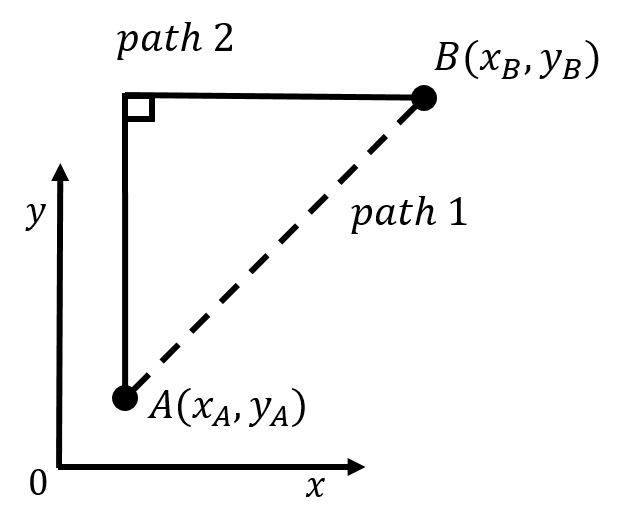
\includegraphics[width=0.4\linewidth]{files/workfriction-1b84b5d4fa9b153b71a19e4b88afa5dc.png}
\caption[]{Two possible paths to slide a crate from position $A$ to position $B$, as seen from above.}
\label{fig:workenergy:workfriction}
\end{figure}

\begin{framed}
\textbf{Solution}\\
The force of kinetic friction is always in the direction opposite to that of motion. Thus, regardless of the path taken, the force of friction will do negative work.

Let us first calculate the work done by the force of kinetic friction along the first path (the straight line). The force of kinetic friction will have a magnitude:
\begin{equation}
f_k = \mu_k N = \mu_k mg
\end{equation}
The normal force will have the same magnitude as the weight because the crate is not moving (accelerating) in the direction perpendicular to the $xy$ plane.  The displacement vector from $A$ to $B$ can be written as:
\begin{equation}
\vec d &= (x_B-x_A)\hat x + (y_B-y_A) \hat y\\
\therefore ||\vec d|| &=d= \sqrt{(x_B-x_A)^2 + (y_B-y_A)^2}
\end{equation}
The force of kinetic friction will be in the opposite direction of the displacement vector, so the angle between the two vectors is $180{\rm \degree}$ ($\cos\theta= -1$). The work done by the force of kinetic friction is thus:
\begin{equation}
W = \vec f_k \cdot\vec d = f_k d \cos\theta = -\mu_k mg\sqrt{(x_B-x_A)^2 + (y_B-y_A)^2}
\end{equation}
and is negative, as expected.

For path 2, we break up the motion into two segments, with displacements vectors $\vec d_1$ (along $y$) and $\vec d_2$ (along $x$). We can write the two displacement vectors as:
\begin{equation}
\vec d_1 &= 0\hat x + (y_B-y_A) \hat y\\
\therefore ||\vec d_1||&=d_1=(y_B-y_A)\\
\vec d_2 &= (x_B-x_A)\hat x + 0 \hat y\\
\therefore ||\vec d_2||&=d_2=(x_B-x_A)\\
\end{equation}
Along each segment, the force of kinetic friction is anti-parallel to the displacement (note that the force of friction changes direction over the two segments), but the magnitude is $f_k=\mu_kmg$. The work done along the first segment is thus:
\begin{equation}
W_1 = \vec f_k \cdot \vec d_1 = f_k d_1 \cos\theta = -\mu_k mg(y_B-y_A)
\end{equation}
The work done along the second segment is:
\begin{equation}
W_2 = \vec f_k \cdot \vec d_2 = f_k d_2 \cos\theta = -\mu_k mg(x_B-x_A)
\end{equation}
And the total work done by the force of kinetic friction over the second path is:
\begin{equation}
W^{tot} = W_1 + W_2 = -\mu_k mg \left((x_B-x_A) + (y_B-y_A)\right)
\end{equation}
which is more work than was done along path 1. This makes sense because for both paths, the force of friction has the same magnitude and is always in the opposite direction of motion; thus, the longer the path, the more work will be done by the force.
\end{framed}
\end{framed}

\begin{framed}
\textbf{Example 7.3}\\
A box of mass $m$ is moved from the floor onto a table using two different paths, as shown in Figure~\ref{fig:workenergy:workgravity}. The table is a horizontal distance $L$ away from where the box starts and a height $H$ above the floor. Compare the work done by the weight of the box along the two possible paths.

\begin{figure}[!htbp]
\centering
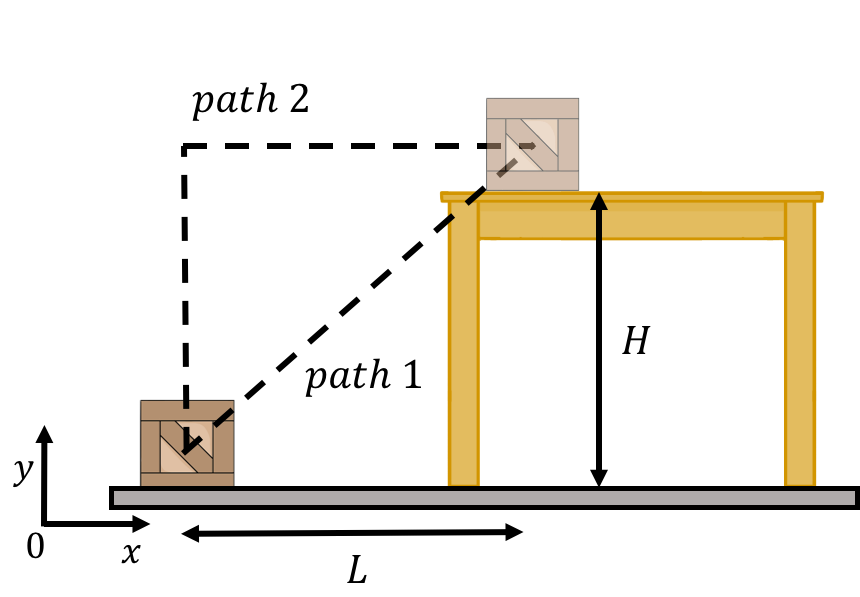
\includegraphics[width=0.5\linewidth]{files/workgravity-875d9fb31a6236f7fd29d3cb33642cbf.png}
\caption[]{Two possible paths to move a box from the floor onto a table.}
\label{fig:workenergy:workgravity}
\end{figure}

\begin{framed}
\textbf{Solution}\\
We can use a coordinate system such that the origin coincides with the initial position of the box. $x$ is horizontal and $y$ is vertical, as shown in Figure~\ref{fig:workenergy:workgravity}. The weight of the box can be written as:
\begin{equation}
\vec F_g = -mg \hat y
\end{equation}
and points in the negative $y$ direction with a magnitude of $mg$. To calculate the work done by the weight along the first path, we first determine the corresponding displacement vector, $\vec d$:
\begin{equation}
\vec d = L\hat x + H\hat y
\end{equation}
and we can then determine the work:
\begin{equation}
W &= \vec F_g \cdot \vec d = (-mg \hat y) \cdot (L\hat x + H\hat y)\\
&=F_xd_x+F_yd_y= (0)(L) + (-mg)(H)\\
&= -mgH
\end{equation}
Along path 1, the work done by the weight is negative, and does not depend on the horizontal distance $L$. Let us now calculate the work done along the second path, which we break up into two segments with displacement vectors $\vec d_1$ (vertical) and $\vec d_2$ (horizontal). The displacement vectors are:
\begin{equation}
\vec d_1 &= H\hat y\\
\vec d_2 &= L\hat x
\end{equation}
The work done along the vertical segment is:
\begin{equation}
W_1 &= \vec F_g \cdot \vec d_1 = (-mg \hat y) \cdot (H\hat y)\\
&=-mgH
\end{equation}
The work done along the horizontal segment is:
\begin{equation}
W_2 &= \vec F_g \cdot \vec d_2 = (-mg \hat y) \cdot (L\hat x)\\
&=0
\end{equation}
which is zero, because the force of gravity is always vertical and thus perpendicular to the displacement vector of the horizontal segment. The total work done by the weight along the second path is:
\begin{equation}
W^{tot} = W_1 + W_2 = -mgH
\end{equation}
which is the same as the work done along path 1. As we will see, when a force is constant in magnitude and direction, the work that it does on an object in going from one position to another is independent of the path taken. This was not the case in Example~7.2, because the direction of the force of kinetic friction depends on the direction of the displacement.
\end{framed}
\end{framed}

\begin{framed}
\textbf{Checkpoint}\\
Clare and Amelia go down two different slides, as shown in Figure~\ref{fig:workenergy:slidecheckpoint}. Clare and Amelia have the same mass and the slides have the same non-zero coefficients of friction.

\begin{figure}[!htbp]
\centering
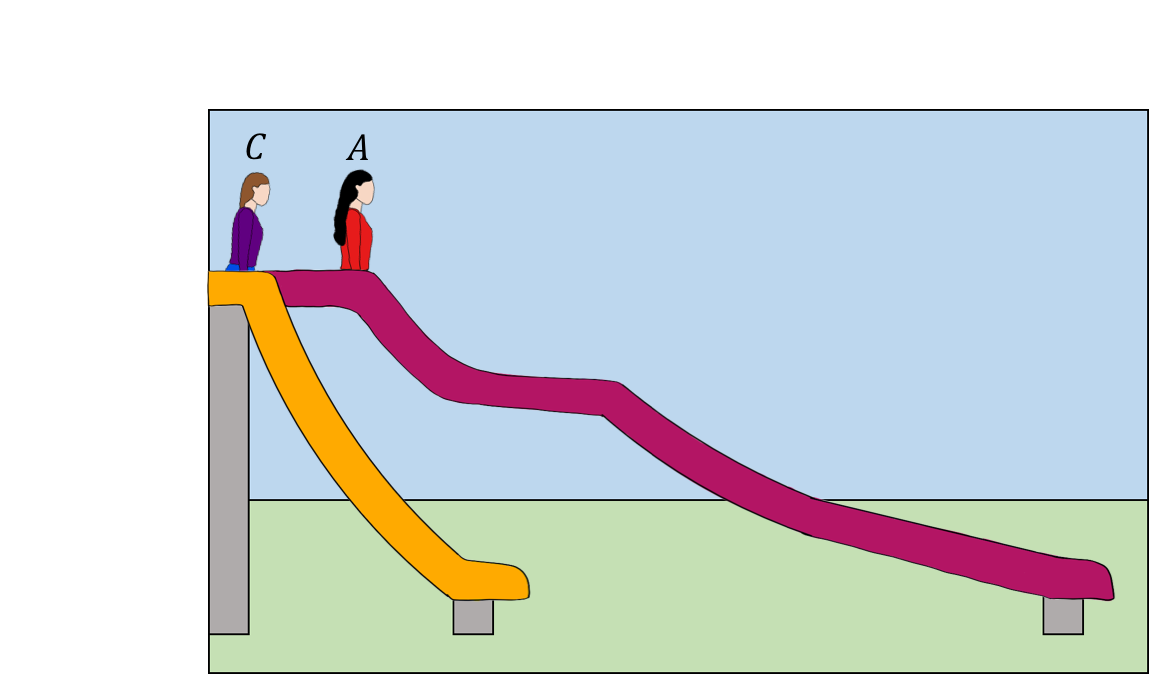
\includegraphics[width=0.5\linewidth]{files/slidecheckpoint-00df72a2d5b8afc63acc302203ecce5c.png}
\caption[]{Clare ($C$) and Amelia ($A$) go down two different slides of the same height.}
\label{fig:workenergy:slidecheckpoint}
\end{figure}

For each of the following forces, decide whether the force: does more work on Clare, does more work on Amelia, or does the same amount of work on both.

\begin{enumerate}
\item The force of gravity...
\item The force of friction...
\item The normal force from the slide...
\end{enumerate}

\begin{framed}
\textbf{Answer}\\
Gravity does the same amount of work on both, friction does more work on Amelia, and the normal force does the same amount of work on both (the normal force does zero work, since it is always perpendicular to the displacement).
\end{framed}
\end{framed}

The most general case for which we can calculate the work done by a force is the case when the force changes continuously along a path where the displacement also changes direction continuously. This is illustrated in Figure~\ref{fig:workenergy:workgeneral} which shows an arbitrary path between two points $A$ and $B$, and a force, $\vec F(\vec r)$, that depends on position ($\vec r$). In general, the work done by the force on an object that goes from $A$ to $B$ will depend on the actual path that was taken.

\begin{figure}[!htbp]
\centering
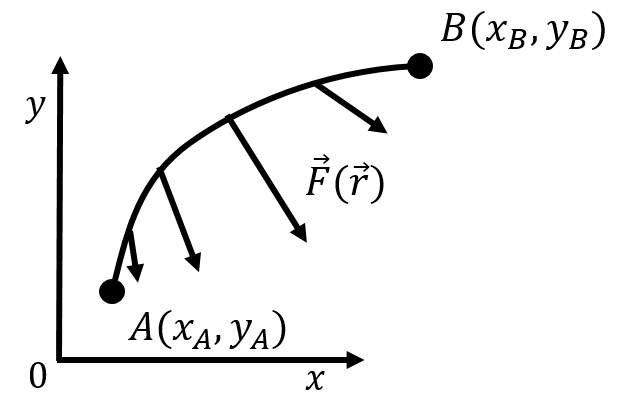
\includegraphics[width=0.5\linewidth]{files/workgeneral-84453b5d1021cea1e90c769f48cf81a0.png}
\caption[]{An arbitrary path between two points $A$ and $B$ with a force that depends on position, $\vec F(\vec r)$.}
\label{fig:workenergy:workgeneral}
\end{figure}

The strategy for calculating the work in the general case is the same: we break up the path into small straight segments with displacement vectors $d\vec l$ (Figure~\ref{fig:workenergy:dldiagram}) where we assume that the force is constant over the segment. The total work is the sum of the work over each segment:
\begin{equation}
\boxed{W = \int_A^B \vec F(\vec r) \cdot d\vec l}
\end{equation}
As usual, we use the integral symbol to indicate that you need to take an infinite number of infinitely small segments $d\vec l$ in order to calculate the sum.

\begin{figure}[!htbp]
\centering
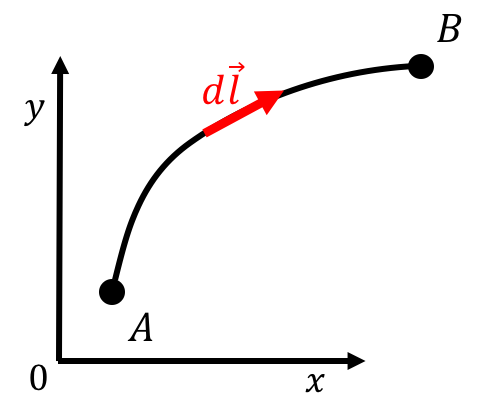
\includegraphics[width=0.3\linewidth]{files/elementoflengthdl-6ada5f90333a0876a91e3ab41ee39190.png}
\caption[]{We divide the path into infinitesimally small segments with displacement vectors $d\vec l$.}
\label{fig:workenergy:dldiagram}
\end{figure}

You should note that this is not an integral like any other that we have seen so far: the integral is not over a single integration variable (usually we use $x$), but it is the integral (the sum!) over the specific path that we have chosen in going from $A$ to $B$. This is called a ``path integral'', and is generally difficult to evaluate.

\begin{framed}
\textbf{Example 7.4}\\
\begin{figure}[!htbp]
\centering
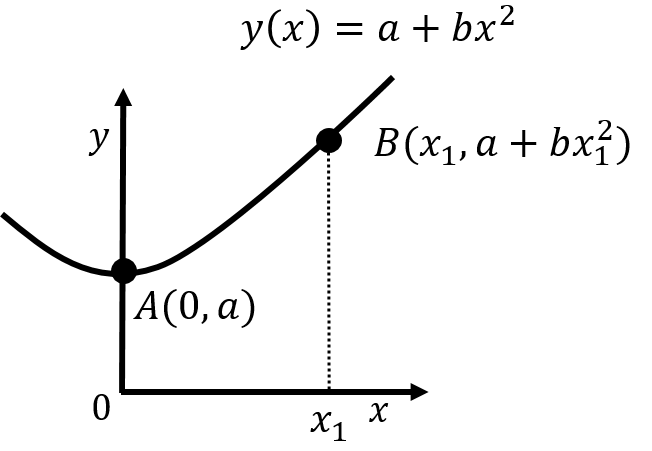
\includegraphics[width=0.4\linewidth]{files/workparabola-d0ed2175e176574cb5fbc15b4d5a2c74.png}
\caption[]{A parabolic path between $A$ and $B$.}
\label{fig:workenergy:workparabola}
\end{figure}

A force, $\vec F(\vec r) = \vec F(x,y) = F_x\hat x + F_y \hat y$,  is exerted on an object. The object starts at position $A$ and ends at position $B$, along a parabolic path, $y(x) = a+bx^2$, as depicted in Figure~\ref{fig:workenergy:workparabola}. What is the work done by the force, $\vec F$, along this trajectory?

\begin{framed}
\textbf{Solution}\\
In this case, the force can change with position (if $F_x$ and $F_y$ are not constant), and the direction of the path changes continuously. When we break up the path into small segments $d\vec l$, we need to incorporate the equation of the parabola to include the fact that $d\vec l$ must always be tangent to the parabola. Consider one small segment along the trajectory and the infinitesimal displacement vector $d\vec l$ at that point, as in Figure~\ref{fig:workenergy:workparabola_dr}.

\begin{figure}[!htbp]
\centering
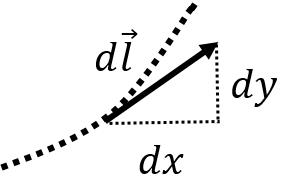
\includegraphics[width=0.3\linewidth]{files/workparabola_dr-759577de91b461f1c08d0dda81a7adc9.png}
\caption[]{The infinitesimal displacement vector, $d\vec l$.}
\label{fig:workenergy:workparabola_dr}
\end{figure}

We can write the $x$ and $y$ components of the vector as infinitesimal distances, $dx$ and $dy$, along the $x$ and $y$ axes, respectively. The vector $d\vec l$ can thus be written:
\begin{equation}
d\vec l = dx \hat x + dy \hat y
\end{equation}
The total work done by the force is then:
\begin{equation}
W &= \int_A^B \vec F(\vec r) \cdot d\vec l\\
&=\int_A^B (F_x\hat x + F_y \hat y) \cdot (dx \hat x + dy \hat y)\\
&=\int_A^B (F_x dx + F_ydy)\\
\therefore W&= \int_A^B F_x dx + \int_A^B F_ydy
\end{equation}
where in the last line, we simply used the property that the integral of a sum is the sum of the corresponding integrals. At this point, we have two integrals over integration variables ($x$ and $y$) that are meaningful. However, we have not yet used the fact that our path is a parabola, and in general, we expect that the shape of the path is important. By saying that we are integrating (or calculating the work) over a specific path, we are really saying that $x$ and $y$ are not independent; that is, if we know the value of $x$ at some point on the path, we know the corresponding value of $y$ ($y = a+bx^2$).

Since $x$ and $y$ are not independent, we can use a ``substitution of variables'' in order to express $y$ in terms of $x$, and $dy$ in terms of $dx$:
\begin{equation}
y(x) &= a + bx^2\\
\frac{dy}{dx} &= 2bx\\
\therefore dy &= 2bxdx
\end{equation}
This allows us to convert the integral over $y$ to an integral over $x$, which also allows us to be explicit for the limits of the integral (in our example, the integral goes from $x=0$ to $x=x_1$):
\begin{equation}
W&= \int_A^B F_x dx + \int_A^B F_ydy\\
&=\int_0^{x_1} F_x dx + \int_0^{x_1} F_y(2bxdx)\\
&=\int_0^{x_1} (F_x + 2bxF_y)dx
\end{equation}
where we would need to know how $F_x$ and $F_y$ depends on $x$ and $y$ in order to actually evaluate the integral.

For example, if the force were constant ($F_x$ and $F_y$ constant), then the work done along the parabolic path would be:
\begin{equation}
W &= \int_0^{x_1} (F_x + 2bxF_y)dx\\
&=\left[F_x x + bF_yx^2  \right]_0^{x_1}\\
&=F_x x_1 + bF_yx_1^2
\end{equation}
As we mentioned earlier, \textbf{if the force is constant in magnitude and direction}, then the work done is independent of path. We can easily check this, using the displacement vector $\vec d = x_1\hat x + bx_1^2 \hat y$:
\begin{equation}
W &= \vec F \cdot \vec d = (F_x\hat x+ F_y\hat y) \cdot (x_1\hat x + bx_1^2 \hat y)\\
&=F_x x_1 + bF_yx_1^2
\end{equation}
as we found above.
\end{framed}
\end{framed}

\paragraph{Net work done}

So far, we have considered the work done on an object by a single force. If more than one force is exerted on an object, then each force can do work on the object, and we can calculate the ``net work'' done on the object by adding together the work done by each force. We will show that this is equivalent to first calculating the net force on the object, $F^{net}$ (i.e. the vector sum of the forces on the object), and then calculating the work done by the net force.

Suppose that three forces, $\vec F_1$, $\vec F_2$, and $\vec F_3$ are exerted on an object as it moves such that its displacement vector is $\vec d$. The net work done on the object is easily shown to be equivalent to the work done by the net force::
\begin{equation}
W^{net} &= W_1 + W_2 + W_3 \\
&= \vec F_1 \cdot \vec d + \vec F_2 \cdot \vec d  + \vec F_3 \cdot \vec d \\
&=(F_{1x}d_x+F_{1y}d_y+F_{1z}d_z)+ (F_{2x}d_x+F_{2y}d_y+F_{2z}d_z) + (F_{3x}d_x+F_{3y}d_y+F_{3z}d_z)\\
&=(F_{1x} + F_{2x} + F_{3x})d_x+(F_{1y} + F_{2y} + F_{3y})d_y+(F_{1z} + F_{2z} + F_{3z})d_z\\
&=\vec F^{net} \cdot \vec d
\end{equation}
where $\vec F^{net} = \vec F_1 + \vec F_2 + \vec F_3$ is the net force. The result is easily generalized to any number of forces, including if those forces change as a function of position:
\begin{equation}
W^{net} = \int_A^B F^{net}(\vec r) \cdot d\vec l
\end{equation}

\begin{framed}
\textbf{Example 7.5}\\
You push with an unknown horizontal force, $\vec F$, against a crate of mass $m$ that is located on an inclined plane that makes an angle $\theta$ with respect to the horizontal, as shown in Figure~\ref{fig:workenergy:workincline}. The coefficient of kinetic friction between the crate and the incline is $\mu_k$. You push in such a way that that crates moves at a constant speed up the incline. What is the net work done on the crate if it moves up the incline by a distance $d$?

\begin{figure}[!htbp]
\centering
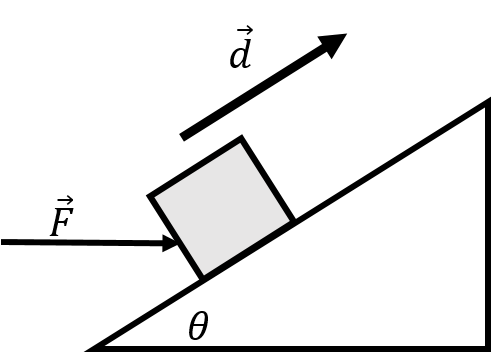
\includegraphics[width=0.3\linewidth]{files/workincline-b98602f6e15a41e5f840950101a04e5d.png}
\caption[]{A crate being pushed up an incline.}
\label{fig:workenergy:workincline}
\end{figure}

\begin{framed}
\textbf{Solution}\\
Although the answer may be obvious, let's go the long way about it and calculate the work done by each force, and then sum them together to get the total work done. We start by identifying the forces exerted on the crate:

\begin{enumerate}
\item $\vec F$, the applied force, of unknown magnitude, $\vec F$.
\item $\vec F_g$, the weight of the crate, with magnitude $mg$.
\item $\vec N$, a normal force exerted by the incline.
\item $\vec f_k$, a force of kinetic friction, with magnitude $\mu_k N$, that points in the direction opposite of $\vec d$.
\end{enumerate}

These are shown in the free-body diagram in Figure~\ref{fig:workenergy:workincline_fbd}, along with our choice of coordinate system, and the displacement vector.

\begin{figure}[!htbp]
\centering
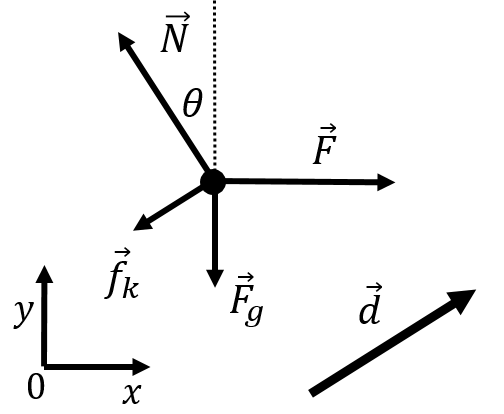
\includegraphics[width=0.3\linewidth]{files/workincline_fbd-7b9ff640523ee3e98aa1d1557bc2919d.png}
\caption[]{Free-body diagram for the crate on the incline.}
\label{fig:workenergy:workincline_fbd}
\end{figure}

With our choice of coordinate system, the displacement vector is given by:
\begin{equation}
\vec d = d (\cos\theta \hat x + \sin\theta \hat y)
\end{equation}
Before calculating the work done by each force, we need to determine the magnitude of the normal force (and thus of the force of kinetic friction). Since the crate is moving at a constant velocity, its \textbf{acceleration is zero}, so the sum of the forces must be zero. Writing out the $y$ component of Newton's Second Law allows us to find the magnitude of the normal force:
\begin{equation}
\sum F_y &= N\cos\theta -F_g - f_k\sin\theta = 0\\
\therefore mg &= N\cos\theta-\mu_kN\sin\theta = N(\cos\theta-\mu_k\sin\theta)\\
\therefore N &= \frac{mg}{\cos\theta-\mu_k\sin\theta}
\end{equation}
Writing out the $x$ component of Newton's Second Law allows us to find the magnitude of the unknown force $F$:
\begin{equation}
\sum F_x &= F - N\sin\theta - f_k\cos\theta = 0\\
\therefore F &= N\sin\theta+\mu_kN\cos\theta = N(\sin\theta+\mu_k\cos\theta)\\
&=mg\frac{\sin\theta+\mu_k\cos\theta}{\cos\theta-\mu_k\sin\theta}
\end{equation}
We now proceed to calculate the work done by each force. The work done by the normal force is identically zero, since it is perpendicular to the displacement vector. The work done by the applied force, $\vec F = F\hat x$, is:
\begin{equation}
W_F &= \vec F \cdot \vec d = (F\hat x)\cdot(d (\cos\theta \hat x + \sin\theta \hat y))\\
&=Fd\cos\theta=mg\frac{\sin\theta+\mu_k\cos\theta}{\cos\theta-\mu_k\sin\theta}d\cos\theta
\end{equation}
The work done by the force of gravity, $\vec F_g = -mg \hat y$, is:
\begin{equation}
W_g &= \vec F_g \cdot \vec d = (-mg \hat y)\cdot(d (\cos\theta \hat x + \sin\theta \hat y))\\
&=-mgd\sin\theta
\end{equation}
The work done by the force of friction, $\vec f_k$, noting that $\vec f_k$ and $\vec d$ are antiparallel:
\begin{equation}
W_f &= \vec f_k \cdot \vec d = -f_kd = -\mu_kNd\\
&=-\mu_k\frac{mg}{\cos\theta-\mu_k\sin\theta}d
\end{equation}
The net work done on the crate is thus:
\begin{equation}
W^{net}&=W_F + W_g + W_f\\
&=mg\frac{\sin\theta+\mu_k\cos\theta}{\cos\theta-\mu_k\sin\theta}d\cos\theta-mgd\sin\theta -\mu_k\frac{mg}{\cos\theta-\mu_k\sin\theta}d\\
&=mgd \left(  \frac{\sin\theta+\mu_k\cos\theta}{\cos\theta-\mu_k\sin\theta}\cos\theta - \sin\theta - \mu_k\frac{1}{\cos\theta-\mu_k\sin\theta} \right)\\
&=mgd \left(  \frac{(\sin\theta+\mu_k\cos\theta)\cos\theta - \sin\theta(\cos\theta-\mu_k\sin\theta) - \mu_k}{\cos\theta-\mu_k\sin\theta} \right)\\
&=mgd \left(  \frac{\sin\theta\cos\theta+\mu_k\cos^2\theta - \sin\theta\cos\theta+\mu_k\sin^2\theta - \mu_k}{\cos\theta-\mu_k\sin\theta} \right)\\
&=mgd \left(  \frac{\mu_k(\cos^2\theta+\sin^2\theta) - \mu_k}{\cos\theta-\mu_k\sin\theta} \right)\\
&=0
\end{equation}
where we used the fact that $\cos^2\theta+\sin^2\theta=1$. Thus we find that the net work done on the crate is zero!

\textbf{Discussion:} Of course, this makes sense, because the net force on the crate is zero, since it is not accelerating, so the net work done is also zero. As a consequence, or rather, by construction, we have the condition that if the net work done on an object is zero, then that object does not accelerate. We thus have a scalar quantity (work) that can tell us something about whether an object is changing speed. In the next section, we introduce a new quantity, ``kinetic energy'', to describe how an object's speed changes when the net work done is not zero.
\end{framed}
\end{framed}

\begin{framed}
\textbf{Olivia's Thoughts}\\
Pay close attention to the words ``on'' and ``by.'' There are a few things about this that can be tricky:

\begin{enumerate}
\item In Example~7.5, we were asked to find the \textbf{net work} done \textbf{on} the crate. Sometimes, the question won't specify that it wants you to find the net work, and will just say ``What is the work done \textbf{on} the crate?'' When you are just asked for the work done ``on'' an object, the question is implicitly asking for the \textit{net} work done on the object.
\item Just because the net work done \textbf{on} an object is zero doesn't mean that the work done \textbf{by} each of the forces is zero. This may seem obvious, but it's easy to get tripped up on a test or exam. If you are reading a question about work and it says that the object is moving at a constant speed, it's tempting to just jump ahead and say that the work must be equal to zero. However, you can only say this if it's asking you for the net work done on the object. For instance, in Example~7.5, we concluded that since the crate was moving at a constant speed, the net work was equal to zero. But if the question asked you to find the work done on the crate \textbf{by gravity}, that would mean something different. The work done \textbf{by gravity} in this case is not equal to zero (it's actually negative).
\item The work done ``on'' an object is not the same as the net work done ``by'' that object. For example, say you are in a tug-of-war and you pull the other team towards you, but you yourself do not move. The net work done \textbf{on} you is zero, but the work done \textbf{by} you is not zero. So, when you are talking about work, you should always state explicitly whether the work is being done ``on'' the object or ``by'' the object.
\end{enumerate}

\textbf{Note}: The wording won't always be like this - sometimes it will say ``How much work do you do on the box?'' instead of ``How much work is done \textbf{by} you on the box,'' so always be careful. Still, looking for key words like ``by'' and ``on'' is a good place to start.
\end{framed}

\begin{framed}
\textbf{Checkpoint}\\
A $2 {\rm kg}$ box sits on a horizontal surface. A constant horizontal force of $6 {\rm N}$ is applied to the box. The box moves with a constant acceleration of $2 {\rm m/s^2}$. Which of the following has the greatest magnitude?

\begin{enumerate}
\item The work done by the applied force.
\item The work done by friction.
\item The net work done on the box.
\end{enumerate}

\begin{framed}
\textbf{Answer}\\
\begin{enumerate}
\item
\end{enumerate}
\end{framed}
\end{framed}

\subsubsection{Kinetic energy and the work energy theorem}\label{sec:workenergy:kinetic}

At this point, you should be comfortable calculating the net work done on an object upon which several forces are exerted. As we saw in the previous section, the net work done on an object is connected to the object's acceleration; if the net force on the object is zero, then the net work done and acceleration are also zero. In this section, we derive a new quantity, kinetic energy, which allows us to connect the work done on an object with its change in speed. This will allow us to describe motion using only scalar quantities. Like the definition of work, the following derivation appears to ``come out of thin air''. Remember, though, that theorists have tried all sorts of mathematical tricks to reformulate Newton's Theory, and this is the one that worked.

Consider the most general case of an object of mass $m$ acted upon by a net force, $\vec F^{net}(\vec r)$, which can vary in magnitude and direction. We wish to calculate the  net work done on the object as it moves along an arbitrary path between two points, $A$ and $B$, in space, as shown in Figure~\ref{fig:workenergy:kepath}. The instantaneous acceleration of the object, $\vec a$, is shown along with an ``element of the path'', $d\vec l$.

\begin{figure}[!htbp]
\centering
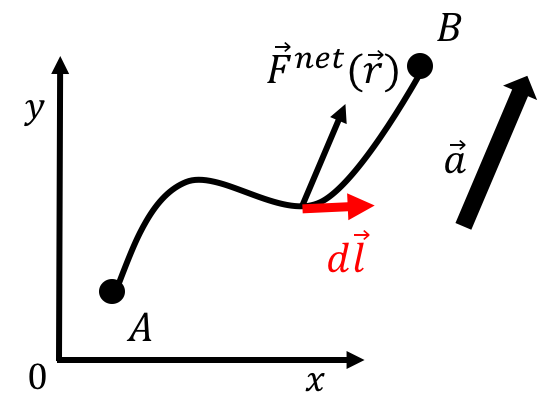
\includegraphics[width=0.4\linewidth]{files/kepath-c0a19725a0d065d2bda035ac72018b9c.png}
\caption[]{An object moving along an arbitrary path between points $A$ and $B$ that is acted upon by a net force $\vec F^{net}$.}
\label{fig:workenergy:kepath}
\end{figure}

The net work done on the object can be written:
\begin{equation}
W^{net} = \int_A^B F^{net}(\vec r) \cdot d\vec l
\end{equation}
and is in general a difficult integral to evaluate for an arbitrary path. Our goal is to find a way to evaluate this integral by finding a function, $K$, with the property that:
\begin{equation}
\int_A^B F^{net}(\vec r) \cdot d\vec l =K_B - K_A
\end{equation}
That is, we will only have to evaluate $K$ at the end points of the path in order to determine the value of the integral. In this way, the function $K$ is akin to an anti-derivative.

In order to determine the form for the function $K$, we start by noting that, by using Newton's Second Law, we can write the integral for work in terms of the acceleration of the object:
\begin{equation}
\sum \vec F &= \vec F^{net} = m\vec a\\
\therefore \int_A^B F^{net}(\vec r) \cdot d\vec l &= \int_A^B m\vec a\cdot d\vec l =m\int_A^B \vec a\cdot d\vec l
\end{equation}
where we assumed that the mass of the object does not change along the path and can thus be factored out of the integral. Consider the scalar product of the acceleration, $\vec a$, and the path element, $d\vec l=dx\hat x  +dy\hat y + dz\hat z$, written in terms of the velocity vector:
\begin{equation}
\vec a & = \frac{d\vec v}{dt}\\
\therefore \vec a\cdot d\vec l &= \frac{d\vec v}{dt}\cdot d\vec l\\
&=\left(\frac{dv_x}{dt}\hat x+ \frac{dv_y}{dt}\hat y + \frac{dv_z}{dt}\hat z\right) \cdot (dx\hat x  +dy\hat y + dz\hat z)\\
&=\frac{dv_x}{dt}dx+\frac{dv_y}{dt}dy+\frac{dv_z}{dt}dz
\end{equation}
Any of the terms in the sum can be re-arranged so that the time derivative acts on the element of path ($dx$, $dy$, or $dz$) instead of the velocity, for example:
\begin{equation}
\frac{dv_x}{dt}dx = \frac{dx}{dt}dv_x
\end{equation}
where we recognize that $\frac{dx}{dt} = v_x$. We can thus write the scalar product between the acceleration vector and the path element as:
\begin{equation}
\vec a\cdot d\vec l&= \frac{dv_x}{dt}dx+\frac{dv_y}{dt}dy+\frac{dv_z}{dt}dz\\
&=\frac{dx}{dt}dv_x + \frac{dy}{dt}dv_y+\frac{dz}{dt}dv_z\\
&=v_xdv_x + v_ydv_y + v_zdv_z
\end{equation}
The integral for the net work done can be written as:
\begin{equation}
W^{net} &= \int_A^B F^{net}(\vec r) \cdot d\vec l =m \int_A^B (v_xdv_x + v_ydv_y + v_zdv_z)\\
&=m\int_A^B v_xdv_x +m\int_A^B  v_ydv_y + m\int_A^B v_zdv_z
\end{equation}
which corresponds to the sum of three integrals over the three independent components of the velocity vector. The components of the velocity vector are functions that change over the path and have fixed values at either end of the path. Let the velocity vector of the object at point $A$ be $\vec v_A=(v_{Ax}, v_{Ay}, v_{Az})$ and the velocity vector at point $B$ be $\vec v_B=(v_{Bx}, v_{By}, v_{Bz})$. The integral over, say, the $x$ component of velocity is then:
\begin{equation}
m\int_A^B v_xdv_x &= m\int_{v_{Ax}}^{v_{Bx}} v_xdv_x= m\left[\frac{1}{2}v_x^2  \right]_{v_{Ax}}^{v_{Bx}}\\
&=\frac{1}{2}m(v_{Bx}^2-v_{Ax}^2)
\end{equation}
We can thus write the net work integral as:
\begin{equation}
W^{net} &=m\int_A^B v_xdv_x +m\int_A^B  v_ydv_y + m\int_A^B v_zdv_z\\
&=\frac{1}{2}m(v_{Bx}^2-v_{Ax}^2) + \frac{1}{2}m(v_{By}^2-v_{Ay}^2) +\frac{1}{2}m(v_{Bz}^2-v_{Az}^2)\\
&=\frac{1}{2}m(v_{Bx}^2+v_{By}^2+v_{Bz}^2)-\frac{1}{2}m(v_{Ax}^2+v_{Ay}^2+v_{Az}^2)\\
&=\frac{1}{2}mv_B^2 - \frac{1}{2}mv_A^2
\end{equation}
where we recognized that the magnitude (squared) of the velocity is given by $v_A^2 = v_{Ax}^2+v_{Ay}^2+v_{Az}^2$. We have thus arrived at our desired result; namely, we have found a function of speed, $K(v)$, that when evaluated at the endpoints of the path allows us to calculate the net work done on the object over that path:
\begin{equation}
\boxed{K(v) = \frac{1}{2}mv^2}
\end{equation}
That is, if you know the speed at the start of the path, $v_A$, and the speed at the end of the path, $v_B$, then the net work done on the object along the path between $A$ and $B$ is given by:
\begin{equation}
\boxed{W^{net} = \Delta K = K(v_B) - K(v_a)}
\end{equation}
We call $K(v)$ the ``kinetic energy'' of the object. We can say that the net work done on an object in going from $A$ to $B$ is equal to its change in kinetic energy (final kinetic energy minus initial kinetic energy). It is important to note that we defined kinetic energy in a way that it is equal to the net work done. You may have already seen kinetic energy from past introductions to physics as a quantity that is just given; here, we instead derived a function that has the desired property of being equal to the net work done and called it ``kinetic energy''.

The relation between the net work done and the change in kinetic energy is called the ``Work-Energy Theorem'' (or Work-Energy Principle). It is the connection that we were looking for between the dynamics (the forces from which we calculate work) and the kinematics (the change in kinetic energy). Unlike Newton's Second Law, which relates two vector quantities (the vector sum of the forces and the acceleration vector), the Work-Energy Theorem relates two scalar quantities to each other (work and kinetic energy). Although we introduced the kinetic energy as a way to calculate the integral for the net work, if you know the value of the net work done on an object, then the Work-Energy Theorem can be used to calculate the change in speed of the object.

Most importantly, the Work-Energy theorem introduces the concept of ``energy''. As we will see in later chapters, there are other forms of energy in addition to work and kinetic energy. The Work-Energy Theorem is the starting point for the idea that you can convert one form of energy into another. The Work-Energy Theorem tells us how a force, by doing work, can provide kinetic energy to an object or remove kinetic energy from an object.

\begin{framed}
\textbf{Example 7.6}\\
A net work of $W$ was done on an object of mass $m$ that started at rest. What is the speed of the object after the work has been done on the object?

\begin{framed}
\textbf{Solution}\\
Using the Work-Energy Theorem:
\begin{equation}
W = \frac{1}{2}mv_f^2 - \frac{1}{2}mv_i^2
\end{equation}
where $v_i$ is the initial speed of the object and $v_f$ is its final speed. Since the initial speed is zero, we can easily find the final speed:
\begin{equation}
v_f = \sqrt{\frac{2W}{m}}
\end{equation}
\end{framed}
\end{framed}

\begin{framed}
\textbf{Example 7.7}\\
A block is pressed against the free end of a horizontal spring with spring constant, $k$, so as to compress the spring by a distance $D$ relative to its rest length, as shown in Figure~\ref{fig:workenergy:spring2}. The other end of the spring is fixed to a wall.

\begin{figure}[!htbp]
\centering
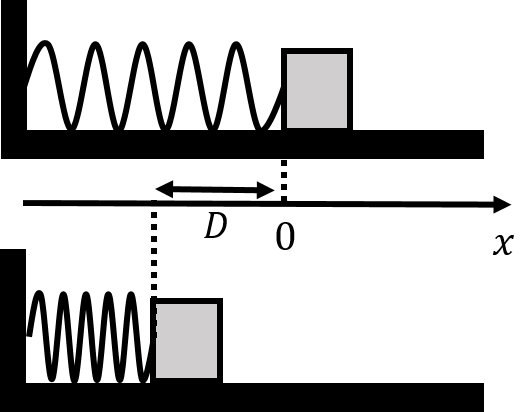
\includegraphics[width=0.4\linewidth]{files/spring-fb0b7b45895ba1ffc941557cc6a32aee.png}
\caption[]{A block is pressed against a horizontal spring so as to compress the spring by a distance $D$ relative to its rest length.}
\label{fig:workenergy:spring2}
\end{figure}

If the block is released from rest and there is no friction between the block and the horizontal surface, what is the speed of the block when it leaves the spring?

\begin{framed}
\textbf{Solution}\\
This is the same problem that we presented in Section~\ref{sec:applyingnewtonslaws:modellingwhereforcechanges} in Example~6.3, where we solved a differential equation to find the speed.

Our first step is to calculate the net work done on the object in going from $x= -D$ to $x=0$ (which corresponds to when the object leaves the spring, as discussed in Example~6.3). The forces on the object are:

\begin{enumerate}
\item $\vec F_g$, its weight, with magnitude $mg$.
\item $\vec N$, the normal force exerted by the ground.
\item $\vec F(x)$, the force from the spring, with magnitude $kx$.
\end{enumerate}

Both the normal force and weight are perpendicular to the displacement, so they will do no work. The net work done is thus the work done by the spring, which we calculated in Example~7.1 to be:
\begin{equation}
W^{net} = W_F = \frac{1}{2}kD^2
\end{equation}
By the Work-Energy Theorem, this is equal to the change in kinetic energy. Noting that the object started at rest ($v_i=0$), the final speed $v_f$ is found to be:
\begin{equation}
W^{net} &=  \frac{1}{2}mv_f^2 - \frac{1}{2}mv_i^2 =  \frac{1}{2}mv_f^2 - 0\\
\frac{1}{2}kD^2 &=\frac{1}{2}mv_f^2\\
\therefore v_f &=\sqrt{\frac{kD^2}{m}}
\end{equation}
\end{framed}
\end{framed}

\begin{framed}
\textbf{Example 7.8}\\
A block is pressed against the free end of a horizontal spring with spring constant, $k$, so as to compress the spring by a distance $D$ relative to its rest length, as shown in Figure~\ref{fig:workenergy:spring3}. The other end of the spring is fixed to a wall.

\begin{figure}[!htbp]
\centering
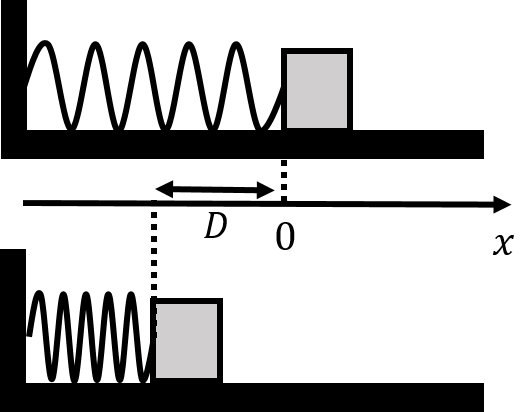
\includegraphics[width=0.4\linewidth]{files/spring-fb0b7b45895ba1ffc941557cc6a32aee.png}
\caption[]{A block is pressed against a horizontal spring so as to compress the spring by a distance $D$ relative to its rest length.}
\label{fig:workenergy:spring3}
\end{figure}

If the block is released from rest and the coefficient of kinetic friction between the block and the horizontal surface is $\mu_k$, what is the speed of the block when it leaves the spring?

\begin{framed}
\textbf{Solution}\\
This is the same example as the previous one, but with kinetic friction. The forces on the block are:

\begin{enumerate}
\item $\vec F_g$, its weight, with magnitude $mg$.
\item $\vec N$, the normal force exerted by the ground on the block.
\item $\vec F(x)$, the force from the spring, with magnitude $kx$.
\item $\vec f_k$, the force of kinetic friction, with magnitude $\mu_kN$.
\end{enumerate}

Both the normal force and weight are perpendicular to the displacement, so they will do no work. Furthermore, since the acceleration in the vertical direction is zero, the normal force will have the same magnitude as the weight ($N=mg$). The magnitude of the force of kinetic friction is thus $f_k = \mu_k mg$. The net work done will be the sum of the work done by the spring, $W_F$, and the work done by friction, $W_f$:
\begin{equation}
W^{net} = W_F + W_f
\end{equation}
We have already determined the work done by the spring:
\begin{equation}
W_F = \frac{1}{2}kD^2
\end{equation}
The work done by the force of kinetic friction will be negative (since it is in the direction opposite of the motion) and is given by:
\begin{equation}
W_f = \vec f_k \cdot \vec d = -f_kD = -\mu_kmgD
\end{equation}
Applying the work energy theorem, and noting that the block started at rest ($v_i=0$), the final speed $v_f$ is found to be:
\begin{equation}
W^{net} =W_F + W_f&= \frac{1}{2}mv_f^2 - \frac{1}{2}mv_i^2 \\
\frac{1}{2}kD^2-\mu_kmgD  &=\frac{1}{2}mv_f^2\\
\therefore v_f &=\sqrt{\frac{kD^2}{m}-2\mu_kgD}
\end{equation}
\textbf{Discussion:} We can think of this in terms of the concept of energy. The spring does positive work on the block, and so it increases its kinetic energy. Friction does negative work on the block, decreasing its kinetic energy. Only the spring is ``introducing'' energy into the block, as friction is removing that energy by doing negative work. Another way to think about it is that the spring is inputting energy; some of that energy goes into increasing the kinetic energy of the block, and some of it is lost by friction.

The energy that is lost to friction can be thought of as ``thermal energy'' (heat) that goes up into heating the block and the surface. Indeed, if you rub your hand against the table, you will notice that it gets warmer; you are losing some of the energy introduced to your hand by the work done by your arm into heating up the table and your hand! This shows that we can think about modelling friction using thermal energy rather than a force.
\end{framed}
\end{framed}

\subsubsection{Power}

We finish the chapter by introducing the concept of ``power'', which is the rate at which work is done on an object, or more generally, the rate at which energy is being converted from one form to another. If an amount of work, $\Delta W$, was done in a period of time $\Delta t$, then the work was done at a rate of:
\begin{equation}
\boxed{P = \frac{\Delta W}{\Delta t}}
\end{equation}
where $P$ is called the power. The SI unit for power is the ``Watt'', abbreviated $\text{W}$, which corresponds to ${\rm J/s}={\rm kg m^2/s^3}$ in base SI units. If the rate at which work is being done changes with time, then the instantaneous power is defined as:
\begin{equation}
\boxed{P = \frac{dW}{dt}}
\end{equation}
You have probably already encountered power in your everyday life. For example, your $1000 {\rm W}$ hair dryer consumes ``electrical energy'' at a rate of $1000 {\rm J}$ per second and converts it into the kinetic energy of the fan as well as the thermal energy to heat up the air. Horsepower ($\text{hp}$) is an imperial unit of power that is often used for vehicles, the conversion being $1 {\rm hp} = 746 {\rm W}$. A $100 {\rm hp}$ car thus has an engine that consumes the chemical energy released by burning gasoline at a rate of $7.46e4 {\rm J}$ per second and converts it into work done on the car as well as into heat.

\begin{framed}
\textbf{Checkpoint}\\
Two cranes lift two identical boxes off of the ground. One crane is twice as powerful as the other. Both cranes do the same amount of work on the boxes and operate at full power. Which of the following statements is true of the boxes, once the cranes have done work on them?

\begin{enumerate}
\item One box has been lifted twice as high as the other.
\item The boxes are lifted to the same height in the same amount of time.
\item The boxes are lifted to the same height, but it takes one of the boxes twice as long to get there.
\item One box is lifted twice as high as the other, but it takes the same amount of time to get there.
\end{enumerate}

\begin{framed}
\textbf{Answer}\\
\begin{enumerate}[resume]
\item
\end{enumerate}
\end{framed}
\end{framed}

\begin{framed}
\textbf{Example 7.9}\\
If a car engine can do work on the car with a power of $P$, what will be the speed of the car at some time $t$ if the car was at rest at time $t=0$?

\begin{framed}
\textbf{Solution}\\
First, we need to calculate how much total work was done on the car:
\begin{equation}
W = P t
\end{equation}
Then, using the Work-Energy Theorem, we can find the speed of the car at some time $t$:
\begin{equation}
W &= \frac{1}{2}mv_f^2 - \frac{1}{2}mv_i^2\\
Pt &= \frac{1}{2}mv_f^2 \\
\therefore v_f &= \sqrt{\frac{2Pt}{m}}
\end{equation}
\textbf{Discussion:} The model for the final speed of the car makes sense because:

\begin{itemize}
\item The dimension of the expression for $v_f$ is speed (you should check this!).
\item The speed is greater if either the time or power are greater (so the speed is larger if more work is done on the car).
\item The speed is smaller if the mass of the car is greater (the acceleration of the car will be less if the mass of the car is larger).
\end{itemize}
\end{framed}
\end{framed}

\begin{framed}
\textbf{Example 7.10}\\
You are pushing a crate along a horizontal surface at constant speed, $v$. You find that you need to exert a force of $\vec F$ on the crate in order to overcome the friction between the crate and the ground. How much power are you expending by pushing on the crate?

\begin{framed}
\textbf{Solution}\\
We need to calculate the rate at which the force, $\vec F$, that you exert on the crate does work. If the crate is moving at constant speed, $v$, then in a time $\Delta t$, it will cover a distance, $d=v\Delta t$. Since you exert a force in the same direction as the motion of the crate, the work done over that distance $d$ is:
\begin{equation}
\Delta W = \vec F \cdot \vec d = Fd\cos(0) = Fv\Delta t
\end{equation}
The power corresponding to the work done in that period of time is thus:
\begin{equation}
P = \frac{\Delta W}{\Delta t} = Fv
\end{equation}
This is quite a general result for the rate at which a force does work when it is exerted on an object moving at constant speed.
\end{framed}
\end{framed}

\begin{framed}
\textbf{Olivia's Thoughts}\\
Example~7.10 ties into what I brought up earlier. If you think to yourself: ``The velocity is constant, so the work must be zero'', the formula,
\begin{equation}
P = \frac{\Delta W}{\Delta t} = Fv
\end{equation}
wouldn't make any sense. Since $v$ is a constant velocity, the power would always be equal to zero, which of course isn't right. Again, remember that when the velocity is constant, it is only the \textbf{net work} that is equal to zero. In Example~7.10, it's asking for the power that \textbf{you} are expending by pushing on the crate (which is the same as asking for the rate of the work done \textbf{by} you \textbf{on} the crate). So, the formula does indeed make sense.
\end{framed}

\subsubsection{Summary}

The work, $W$, done on an object by a force, $\vec F$, while the object has moved through a displacement, $\vec d$, is defined as the scalar product:
\begin{equation}
W = \vec F \cdot \vec d &= Fd\cos\theta\\
&= F_xd_x+F_yd_y+F_zd_z
\end{equation}
If the force changes with position and/or the object moves along an arbitrary path in space, the work done by that force over the path is given by:
\begin{equation}
W =\int_A^B \vec F(\vec r) \cdot  d\vec l
\end{equation}
% Work allows us to quantify how a force acting on an object changes the speed of that object.

If multiple forces are exerted on an object, then one can calculate the net force on the object (the vector sum of the forces), and the net work done on the object will be equal to the work done by the net force:
\begin{equation}
W^{net} = \int_A^B \vec F^{net}(\vec r) \cdot d\vec l
\end{equation}
If the net work done on an object is zero, that object does not accelerate.

We can define the kinetic energy, $K(v)$ of an object of mass $m$ that has speed $v$ as:
\begin{equation}
K(v) = \frac{1}{2} mv^2
\end{equation}

The Work-Energy Theorem states that the net work done on an object in going from position $A$ to position $B$ is equal to the object's change in kinetic energy:
\begin{equation}
W^{net} = \Delta K = \frac{1}{2} mv_B^2 - \frac{1}{2} mv_A^2
\end{equation}
where $v_A$ and $v_B$ are the speed of the object at positions $A$ and $B$, respectively.

The rate at which work is being done is called power and is defined as:
\begin{equation}
P = \frac{dW}{dt}
\end{equation}
If a constant force $\vec F$ is exerted on an object that has a constant velocity $\vec v$, then the power that corresponds to the work being done by that force is:
\begin{equation}
P &= \frac{d}{dt} W = \frac{d}{dt}(\vec F \cdot \vec d)\\
&= \vec F \cdot \frac{d}{dt}\vec d = \vec F \cdot \vec v
\end{equation}

\begin{framed}
\textbf{Important Equations}\\
\textbf{Work:}
\begin{equation}
W &= \vec F \cdot \vec d = Fd\cos\theta\\
W &= F_xd_x+F_yd_y+F_zd_z\\
W &=\int_A^B \vec F(\vec r) \cdot  d\vec l\\
W^{net} &= \int_A^B \vec F^{net}(\vec r) \cdot d\vec l
\end{equation}
\textbf{Kinetic Energy:}
\begin{equation}
K(v) = \frac{1}{2} mv^2
\end{equation}

\textbf{Work-Energy Theorem:}
\begin{equation}
W^{net} = \Delta K = \frac{1}{2} mv_B^2 - \frac{1}{2} mv_A^2
\end{equation}
\textbf{Power:}
\begin{equation}
P &= \frac{dW}{dt}\\
P &= \vec F \cdot \vec v
\end{equation}
\end{framed}

\begin{framed}
\textbf{Important Definitions}\\
\begin{itemize}
\item \textbf{Kinetic energy:} A form of energy that an object with a mass has by virtue of having a non-zero speed. SI units: [{\textbackslash}text\{J\}]. Common variable(s): $K$.
\item \textbf{Power:} The rate at which energy is converted with respect to time. SI units: ${\rm \left[{W}\right]}$. Common variable(s): $P$.
\end{itemize}
\end{framed}

\subsubsection{Thinking about the material}

\begin{framed}
\textbf{Reflect and research}\\
\begin{itemize}
\item When was the concept of work first introduced?
\item To construct the pyramids, the ancient Egyptians used simple machines, like levers, to accomplish tasks that would not be possible otherwise. Apply what we know about work to find out how levers help people lift incredibly heavy objects.
\item After an accident, investigators use skid marks to figure out how fast the cars were going before the crash. Use your knowledge of work, figure out how they do this.
\item The Tesla Model S can accelerate from 0-100 {\textbackslash}si\{km/h\} in as little as 2.7 seconds. Calculate the power of the car in horsepower. Why is it unusual for a 7 seat sedan, like the Model S, to have such a short acceleration time? Investigate how it's possible for the Tesla to accelerate so quickly.
\end{itemize}
\end{framed}

\begin{framed}
\textbf{To try at home}\\
\begin{itemize}
\item Measure the power that you can output with your legs, and describe how you made the measurement.
\end{itemize}
\end{framed}

\begin{framed}
\textbf{To try in the lab}\\
\begin{itemize}
\item Propose an experiment to measure the thermal energy associated with a force of kinetic friction.
\item Propose an experiment to test the Work-Energy Theorem.
\end{itemize}
\end{framed}

\subsubsection{Sample problems and solutions}

\paragraph{Problems}

\begin{framed}
\textbf{Problem 7.1}\\
A ski jump can is modelled as a ramp of height $h=5 {\rm m}$, as shown in Figure~\ref{fig:workenergy:skijumpprob}. The landing area is at the same height as the bottom of the ramp. A skier of mass $m=80 {\rm kg}$ is moving at a speed $v_i=15 {\rm m/s}$ when they reach the bottom of the ramp. When the skier lands the jump, their speed is measured to be $v_f=12 {\rm m/s}$. Ignore air resistance.

\begin{figure}[!htbp]
\centering
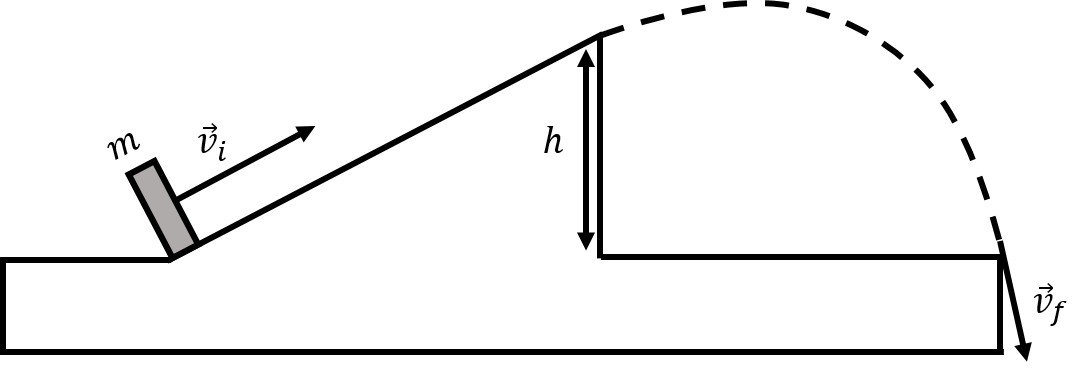
\includegraphics[width=0.7\linewidth]{files/skijumpprob-7a4485948f1dc2b2671e28671fec477f.png}
\caption[]{A person of mass $m$ goes off a ski jump of height $h$.}
\label{fig:workenergy:skijumpprob}
\end{figure}

\begin{itemize}
\item a. What is the speed of the skier the instant they leave the ski jump, at the top of the ramp?
\item b. Use the answer from part (a) to find the work done by the force of friction between the ramp and the skier.
\end{itemize}
\end{framed}

\begin{framed}
\textbf{Problem 7.2}\\
A child of mass $m$ sits on a swing of length $L$, as in Figure~\ref{fig:workenergy:swingprob}. You push the child with a horizontal force $\vec F$. You apply the force in such a way that the child moves at a constant speed (note that $\vec F$ will not have a constant magnitude).\}

\begin{itemize}
\item a. How much work do you do to move the child from $\theta=0$ to $\theta=\theta_1$?
\item b.  Use a detailed diagram to show that the work done by $\vec F$ is equal to $mgh$, where $h$ is the change in height of the child.
\end{itemize}

\begin{figure}[!htbp]
\centering
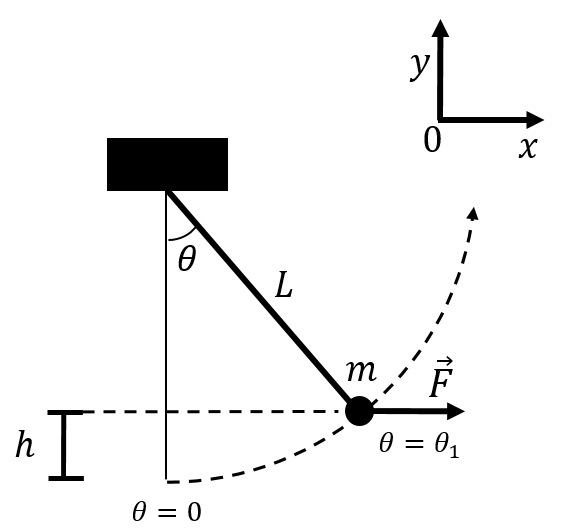
\includegraphics[width=0.4\linewidth]{files/swingprob-d71c20d72bf5df16dc390c24266b1394.png}
\caption[]{A child on a swing is pushed from $\theta=0$ to $\theta=\theta_1$ at constant speed with a horizontal force, $\vec F$.}
\label{fig:workenergy:swingprob}
\end{figure}
\end{framed}

\paragraph{Solutions}

\begin{framed}
\textbf{Solution}\\
\begin{itemize}
\item a. We start by defining a coordinate system. We choose the $x$ axis to be horizontal and positive in the direction of motion, and we choose the $y$ axis to be vertical and the positive direction upwards.
\end{itemize}

We will determine the speed at the top of the ramp, $v_t$, using the Work-Energy Theorem:
\begin{equation}
W^{net}=\frac{1}{2}mv_f^2-\frac{1}{2}mv_t^2
\end{equation}
where $W^{net}$ is the net work done on the skier as they ``fly'' through the air. While the skier is in the air, the only force acting on them is gravity, $\vec F= -mg\hat y$. The path of the skier is a parabola, so that the displacement vector changes direction continuously. The work done by gravity is given by:
\begin{equation}
W = \int \vec F_g \cdot d\vec l
\end{equation}
where $d\vec l$ is an infinitesimal displacement along the trajectory, as shown in Figure~\ref{fig:workenergy:skiprobdisplacement}.

\begin{figure}[!htbp]
\centering
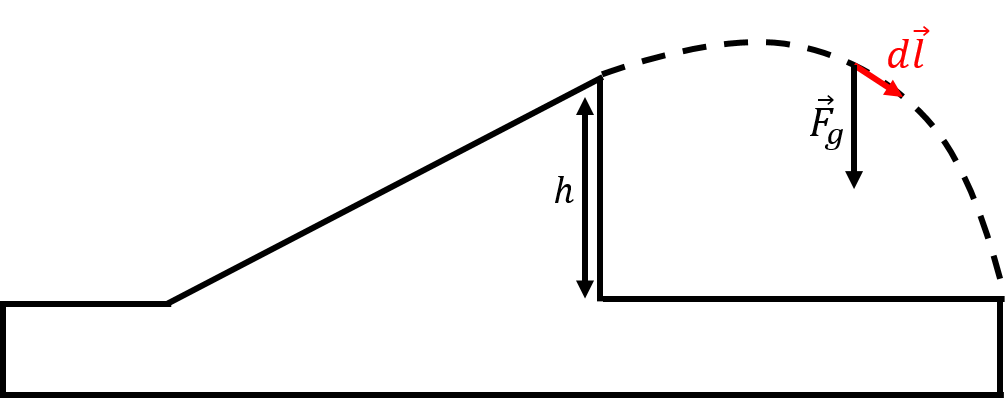
\includegraphics[width=0.7\linewidth]{files/skiprobdisplacement-89a036a287b9d6e9cdb4ce44a58e8c29.png}
\caption[]{Infinitesimal displacement along the trajectory of the jump.}
\label{fig:workenergy:skiprobdisplacement}
\end{figure}

The displacement vector will have $x$ and $y$ components:
\begin{equation}
d\vec l = dx \hat x + dy \hat y
\end{equation}
The scalar product with the force of gravity is thus:
\begin{equation}
\vec F_g \cdot d\vec l &= (-mg\hat y) \cdot (dx \hat x + dy \hat y)= -mgdy
\end{equation}
The work done by gravity can thus be converted into an integral over $y$ (for which we know the start and end values), and is given by:
\begin{equation}
W = \int \vec F_g \cdot d\vec l = \int_h^0 -mgdy = [-mgy]_h^0 = mgh
\end{equation}
The work done by gravity is positive, which makes sense, since the force of gravity is generally in the same direction as the net displacement (downwards). We did not need to take into account the specific shape of the trajectory, because the force was constant in magnitude and direction (see Example~7.4).

We can now find the speed of the skier when they leave the jump using the Work-Energy theorem:
\begin{equation}
W^{net}&=\frac{1}{2}mv_f^2-\frac{1}{2}mv_t^2\\
mgh &= \frac{1}{2}mv_f^2-\frac{1}{2}mv_t^2\\
\therefore v_t&=\sqrt{v_f^2-2gh}=\sqrt{(12 {\rm m/s})^2 - 2(9.8 {\rm m/s^2})(5 {\rm m})}=6.8 {\rm m/s}
\end{equation}

\begin{itemize}
\item b. We can again use the Work-Energy Theorem to determine the work done by friction as the skier slides up the ramp. We know that the speed of the skier at the bottom of the ramp is $v_i$, and we just found that the speed of the skier at the top of the ramp is $v_t=\sqrt{v_f^2 -2gh}$. The net work done on the skier going up the ramp is equal to:
\end{itemize}
\begin{equation}
W^{net}&=\frac{1}{2}mv_t^2-\frac{1}{2}mv_i^2\\
&=\frac{1}{2}m(v_t^2-v_i^2) = \frac{1}{2}m(v_f^2-2gh -v_i^2)\\
&=\frac{1}{2}m(v_f^2-v_i^2)-mgh
\end{equation}
The net work done is also the sum of the work done by each of the forces acting on the skier as they slide up the ramp. The forces on the skier are the force of gravity, the force of friction, and the normal force. The normal force does no work, since it is always perpendicular to the displacement. The net work is thus the sum of the work done by the force gravity, $W_g$, and the work done by the force of friction, $W_f$, over the displacement corresponding to the length of the ramp:
\begin{equation}
W^{net}=W_g+W_f
\end{equation}
The work done by gravity is:
\begin{equation}
W_g = \vec F_g \cdot \vec d = (-mg\hat y) \cdot  (d_x\hat x + h \hat y) = -mgh
\end{equation}
where $\vec d$ is the displacement vector up the ramp (unknown horizontal distance, $d_x$, and vertical distance, $h$). We can now determine the work done by the force of friction:
\begin{equation}
W^{net}&=W_g+W_f\\
\frac{1}{2}m(v_f^2-v_i^2)-mgh &=  -mgh + W_f\\
\therefore W_f &= \frac{1}{2}m(v_f^2-v_i^2) = \frac{1}{2}(80 {\rm kg})((12 {\rm m/s})^2-(15 {\rm m/s})^2)=-3240 {\rm J}
\end{equation}
And we find that the force of friction did negative work (it reduced the kinetic energy of the skier).

\textbf{Discussion:} Over the course of the jump, the skier started at the bottom of the ramp with a given kinetic energy, then lost some of that energy going up the ramp (in the form of loss to friction and negative work done by gravity). During the airborne phase, gravity did positive work and the skier gained back some of the kinetic energy that they had lost going up the ramp. Thus the net work done by the force of friction is the difference in kinetic energies between the final landing point and the beginning of the ramp, because friction is the only force that did a net amount of (negative) work over the whole trajectory (gravity did no net work over the whole trajectory). This example shows how we can start to think about energy as something that is ``conserved'', which we will explore in more detail in the next chapter.
\end{framed}

\begin{framed}
\textbf{Solution}\\
\begin{itemize}
\item a. We want to find the work done by the applied force $\vec F$. We first need to find an expression for the magnitude of $\vec F$, based on the fact that the child is not accelerating. The forces on the child are:
\item $\vec F_g$, their weight, with magnitude $mg$.
\item $\vec F_T$, the tension in the rope, which changes with the angle, $\theta$.
\item $\vec F$, the applied force, which change in magnitude as the angle, $\theta$, changes.
\end{itemize}

The forces are illustrated in Figure~\ref{fig:workenergy:swingprobfbd}.

\begin{figure}[!htbp]
\centering
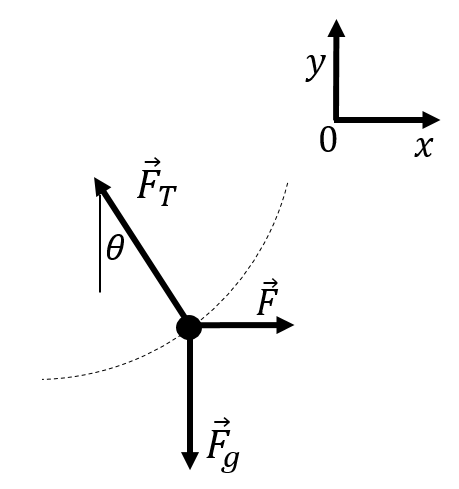
\includegraphics[width=0.3\linewidth]{files/swingprobfbd-ba84c7450092567037aea8b370051104.png}
\caption[]{A free-body diagram of the forces exerted on the child.}
\label{fig:workenergy:swingprobfbd}
\end{figure}

The child is moving at a constant speed, so the net force is equal to zero. The sum of the $x$ and $y$ components of the forces are equal to zero (Newton's Second Law):
\begin{equation}
\sum F_x &= F-F_T\sin\theta =0\\
\sum F_y &= F_T\cos\theta -mg = 0
\end{equation}
Rearranging these equations gives:
\begin{equation}
F&=F_T\sin\theta\\
mg&=F_T\cos\theta
\end{equation}
We want an expression for $F$ that does not depend on $F_T$ (since $F_T$ is unknown), so we can divide one equation by the other:
\begin{equation}
\frac{F}{mg} &= \frac{F_T\sin\theta}{F_T\cos\theta}=\tan\theta\\
\therefore F(\theta)&=mg\tan\theta
\end{equation}
where we indicated that the force $\vec F(\theta)$ depends on the angle $\theta$. The work done by the force, $\vec F$, is given by:
\begin{equation}
W_F=\int_A^B\vec F(\theta) \cdot d\vec l
\end{equation}
$d\vec l$ is the ``path element'' along part of the arc of circle over which the child moves, as illustrated in Figure~\ref{fig:workenergy:swingprobdl}. We have an expression for how $\vec F$ changes in magnitude as a function of the angle $\theta$, and it would thus be convenient to perform the integral over the angle $\theta$.

\begin{figure}[!htbp]
\centering
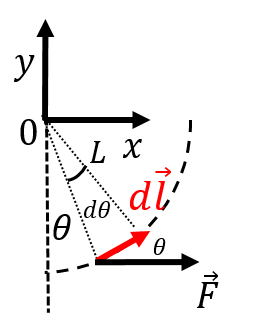
\includegraphics[width=0.2\linewidth]{files/swingprobdl-adf6f6b05a5bd3d9b8b20443ef022b01.png}
\caption[]{A path element along the circular trajectory of the swing.}
\label{fig:workenergy:swingprobdl}
\end{figure}

We can use polar coordinate, $(r,\theta)$, instead of cartesian coordinates to describe the displacement vector, $d\vec l$. If the vector subtends an arc on the circle that makes an infinitesimal angle, $d\theta$, as illustrated, then the length of the vector $d\vec l$ is given by:
\begin{equation}
dl = L d\theta
\end{equation}
where $L$ is the radius of the circle. The vector $d\vec l$ makes an angle $\theta$ with the horizontal, and thus with the vector, $\vec F$. The dot product between $\vec F$ and $d\vec l$ can thus be written as:
\begin{equation}
\vec F(\theta) \cdot d\vec l = Fdl\cos\theta=(mg\tan\theta)(Ld\theta)\cos\theta=mgL\sin\theta d\theta
\end{equation}
We can now write the integral for the work using limit that are based on the angle $\theta$, from $\theta=0$ to $\theta=\theta_1$:
\begin{equation}
W&=\int_0^{\theta_1}mgL\sin\theta d\theta\\
&=mgL[-\cos\theta]_0^{\theta_1}=mgL(1-\cos\theta_1)
\end{equation}

\begin{itemize}
\item b. We know that the work done by $\vec F$ is $W=mgL(1 -\cos\theta_1)$. So, we want to prove that $L(1 -\cos\theta_1)$ is equal to $h$. Expanding $L(1 -\cos\theta_1)$ gives:
\end{itemize}
\begin{equation}
L(1-\cos\theta_1)&=L-L\cos\theta_1
\end{equation}
This can be illustrated on a diagram, as in Figure~\ref{fig:workenergy:swingprobgeometry}, which shows that $h$ is equal to $L -L\cos\theta$.

\begin{figure}[!htbp]
\centering
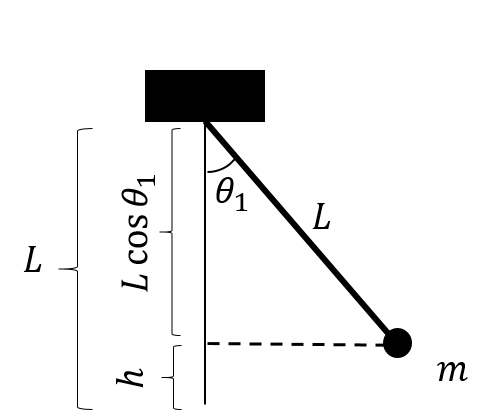
\includegraphics[width=0.4\linewidth]{files/swingprobgeometry-0ebc2108f22acceabc86359d39684055.png}
\caption[]{A diagram showing the geometry of the problem}
\label{fig:workenergy:swingprobgeometry}
\end{figure}

\textbf{Discussion:} The net force acting on the mass is equal to zero, so the net work must be equal to zero. The two forces that do work on the mass are the applied force $\vec F$, and gravity. The work done by the applied force if $mgh$, so the work done by gravity must be $-mgh$.
\end{framed}